\chapter{Methodology}

\section{Target}
This thesis focuses on drug perturbation prediction. Let $G$ be the number of genes in the selected gene set. Assuming that a single paired sample consists of a matched control profile $x_{\mathrm{ctl}} \in \mathbb{R}^{G}$ and a treated profile $x_{\mathrm{trt}} \in \mathbb{R}^{G}$, the supervised training target is defined as their difference:
\begin{equation}
y = x_{\mathrm{trt}} - x_{\mathrm{ctl}} \in \mathbb{R}^{G}.
\end{equation}
Accordingly, the objective of our models is to output a predicted response vector $\hat{y} \in \mathbb{R}^{G}$.

\noindent When processed in a mini-batch of size $B$, the target tensor has the shape $Y \in \mathbb{R}^{B \times G}$ and the corresponding model prediction has the shape $\hat{Y} \in \mathbb{R}^{B \times G}$.

\section{Inputs}
\noindent Each training instance combines three main components: a matched control profile, a drug representation, and optional cell context information. To ensure consistency across different model variants, these inputs are mapped row by row to individual paired conditions and aligned by gene order across the control profile, the drug target vector, and the final predicted response.

\subsection{Control data}
The primary sample-level input is the matched control profile $x_{\mathrm{ctl}} \in \mathbb{R}^{G}$. In simple terms, this vector shows the natural, baseline state of the cell before any drug is applied. Supplying this measurement as a direct input is important because the same drug can act very differently depending on the starting condition of the cell. A drug's effect relies heavily on which genes are already turned on and which biological pathways are currently active. By looking at this initial baseline, the neural network can tune its predictions to account for the natural differences between various cell types and experiments.

\noindent In our main setup, we use $G=978$ landmark genes, meaning each control sample is represented as a 978-dimensional vector of continuous numbers. For a mini-batch of size $B$, the control input tensor has the shape $X_{\mathrm{ctl}} \in \mathbb{R}^{B \times G}$. As illustrated in Figure~\ref{fig:ctl_node_projection}, these measured values map directly to the nodes in our graph model. The network takes the initial scalar value for each gene and projects it to serve as the starting mathematical feature for that specific gene node. This ensures that the graph network bases its early calculations on real biological measurements before the nodes start sharing information with each other.

\begin{figure}[H]
    \centering
    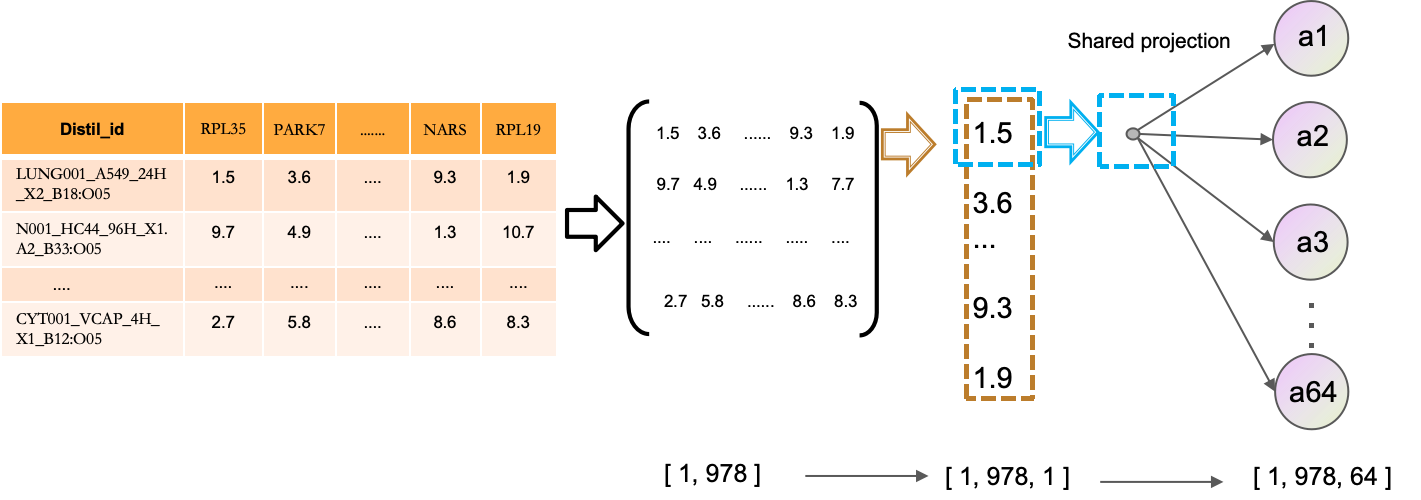
\includegraphics[width=0.95\linewidth]{figures/per_node_ctl_input.png}
    \caption{Control input and its node wise projection. Each sample is represented as a 978 dimensional gene expression vector aligned to the gene order. The same shared projection layer maps each gene wise scalar input to a 64 dimensional node feature.}
    \label{fig:ctl_node_projection}
\end{figure}

\subsection{Drug target}
The primary drug input, denoted as $x_{\mathrm{drug}} \in \mathbb{R}^{G}$, is a binary target vector aligned to the strict gene order. An entry in this vector is set to one if the corresponding gene is an annotated target of the drug, and zero otherwise. While extra molecular fingerprint vectors could be supplemented in certain model variants, the main benchmark in this thesis solely relies on this target-based vector. For a mini-batch, the drug input spans a shape of $X_{\mathrm{drug}} \in \mathbb{R}^{B \times G}$.

\begin{figure}[H]
    \centering
    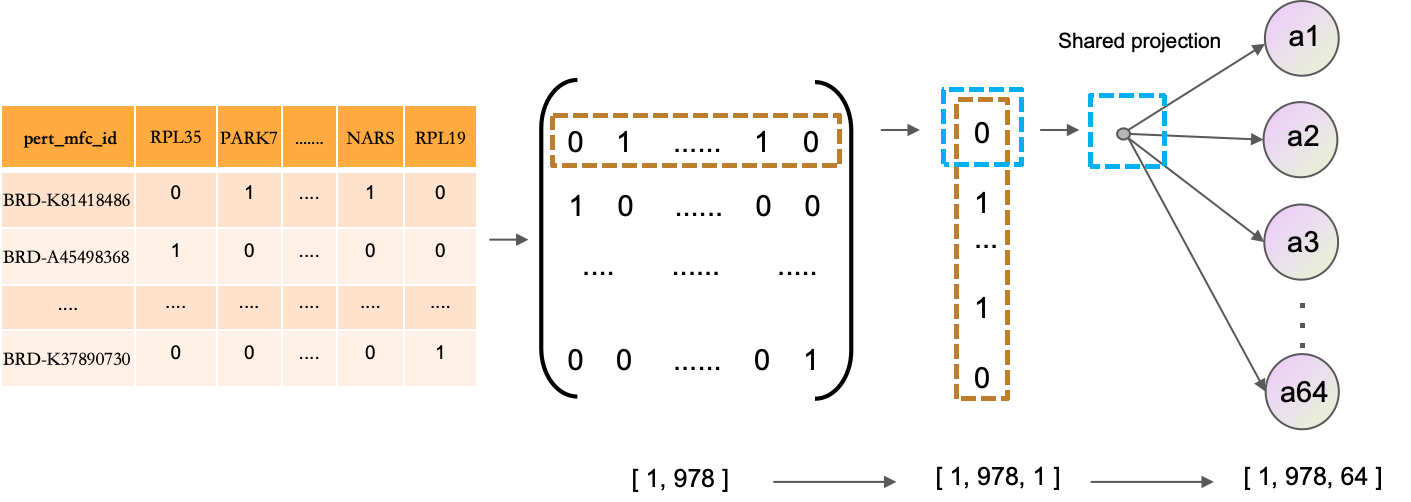
\includegraphics[width=0.95\linewidth]{figures/per_node_drug_input.png}
    \caption{Drug target input and its node wise projection. Each sample is represented as a binary target vector aligned to the gene order. After adding a singleton feature dimension, the same shared projection layer maps each gene wise scalar input to a 64 dimensional node feature.}
    \label{fig:drug_target_projection}
\end{figure}

\subsection{Biological graph}
The proposed architecture integrates prior biological knowledge via a directed graph $\mathcal{G}=(\mathcal{V},\mathcal{E})$ derived from the OmniPath database. Given that each node corresponds to a gene in the selected set, the absolute bounds of the vertices equate to the constant $G$. The graph is formalized as a directed adjacency matrix $A \in \mathbb{R}^{G \times G}$.

\noindent This adjacency matrix efficiently encodes both the existence and the regulatory sign of an interaction. Specifically, the column index denotes the source gene ($u$) and the row index denotes the target gene ($v$). If gene $u$ stimulates gene $v$, the entry $A_{vu}$ is positive; if it acts as an inhibitor, the entry is negative; and if no regulatory edge exists between them, the connection remains zero.

\subsection{Cell information}
Inspired by recent context-aware perturbation models like GSNN and XPert~\cite{evans2024gsnn,guo2026xpert}, this study considers two separate paradigms to incorporate cellular state and metadata to improve prediction accuracy.

\noindent The first approach utilizes a cell identity embedding, which assigns a single learned vector in $\mathbb{R}^{F}$ to a specific cell line. While this fixed-label design is easy to optimize and serves as our default benchmark configuration, it indiscriminately broadcasts the identical representation to all gene nodes across all samples originating from that cell line.

\begin{figure}[H]
    \centering
    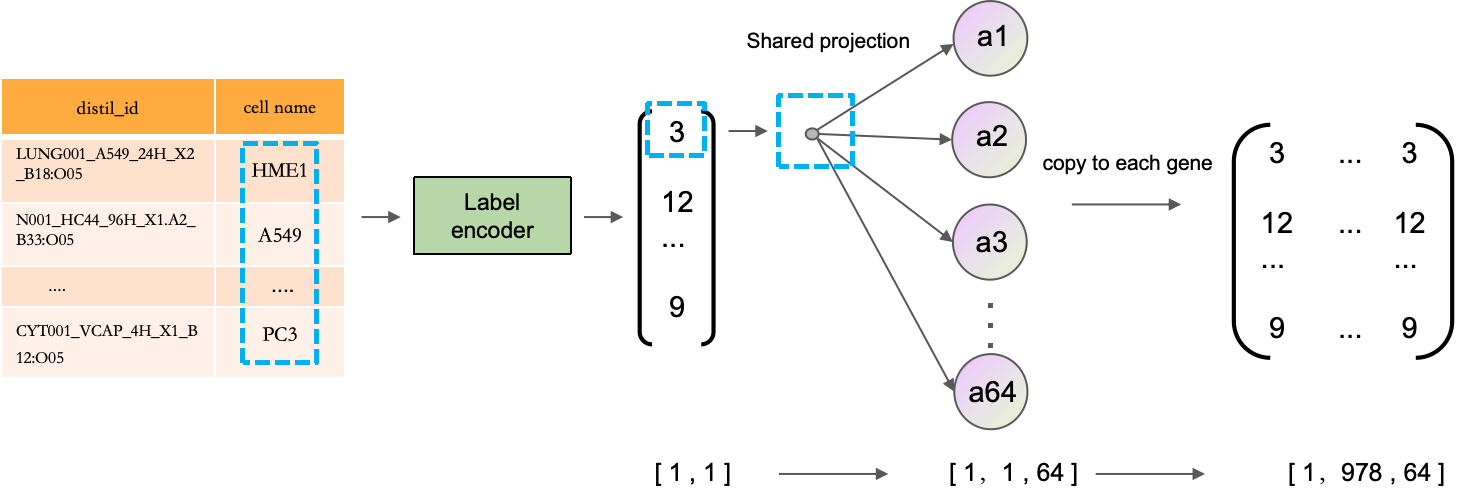
\includegraphics[width=0.95\linewidth]{figures/cellid_input.png}
    \caption{Cell identity input and its embedding. Each cell line name is first mapped to an integer index by a label encoder, and then a learnable embedding layer maps the index to a 64 dimensional cell representation. The same cell embedding is shared by all samples from the same cell line.}
    \label{fig:cellid_embedding}
\end{figure}

\noindent The second approach leverages a control-derived cell context. This relies on the premise that the matched control profile serves as a direct observation of the sample before the drug perturbation is introduced. Because its expression pattern intrinsically captures the sample-specific baseline state, reflecting active genes, silent pathways, and intra-cell-line variations, the full control profile $x_{\mathrm{ctl}}$ can be dynamically encoded rather than treating the cell state as a static label. Formally, $x_{\mathrm{ctl}}$ is normalized and processed through a latent encoder to yield a robust, sample-specific context vector $c_{\mathrm{ctx}} \in \mathbb{R}^{F}$.

\begin{figure}[H]
    \centering
    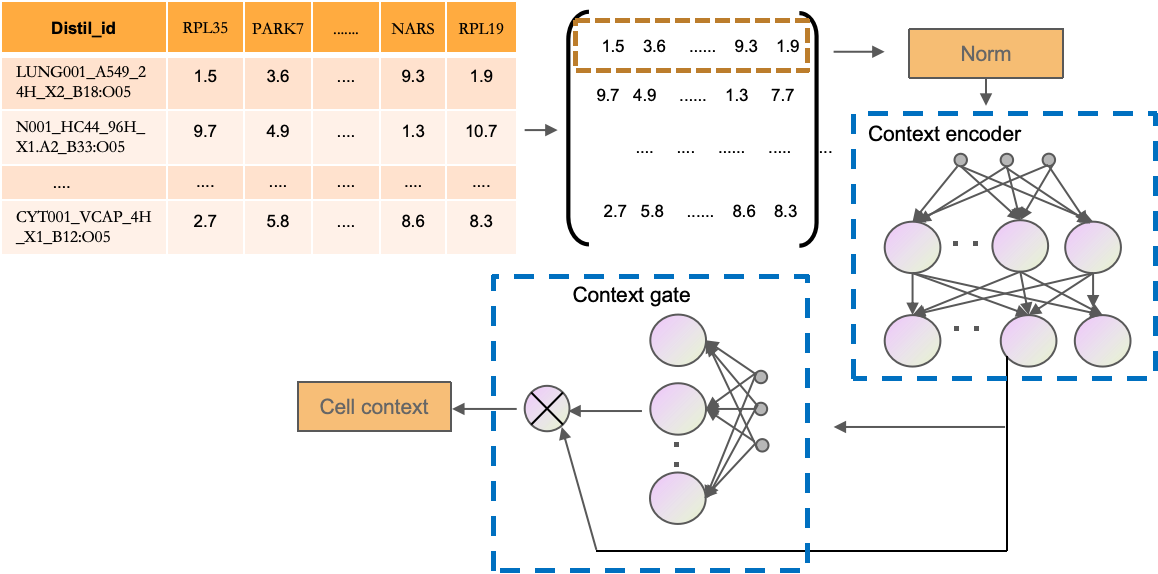
\includegraphics[width=0.95\linewidth]{figures/cell_context.png}
    \caption{Control derived cell context. The control profile is normalized and encoded into a sample specific context vector. This context summarizes the baseline expression state of the sample before drug perturbation.}
    \label{fig:cell_context}
\end{figure}

\noindent To maximize the advantages of both designs, we introduce a hybrid setting that fuses both sources of cell information. The fixed cell identity is first mapped to its learned embedding $c_{\mathrm{id}} \in \mathbb{R}^{F}$. A final sample-level cell representation is then constructed by fusing it with the dynamic context:
\begin{equation}
c_{\mathrm{fused}} = \alpha_{\mathrm{id}} c_{\mathrm{id}} + \alpha_{\mathrm{ctx}} c_{\mathrm{ctx}},
\end{equation}
where $\alpha_{\mathrm{id}}$ is a learnable scalar weight that dictates the trade-off, and $\alpha_{\mathrm{ctx}} = 1 - \alpha_{\mathrm{id}}$. This unified formulation seamlessly combines a coarse prior for the general cell type with a highly sample-specific correction dictated by the observed baseline expression measurements.

\begin{figure}[H]
    \centering
    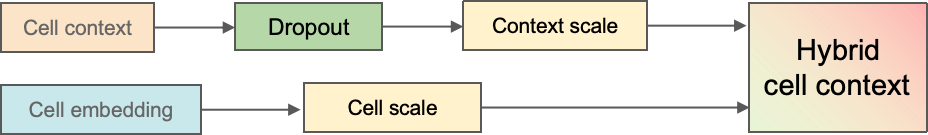
\includegraphics[width=0.79\linewidth]{figures/Hybrid_cell_context.png}
    \caption{Hybrid cell context fusion. The cell identity embedding and the control derived context are scaled and combined into one fused sample level representation.}
    \label{fig:hybrid_cell_context}
\end{figure}

\noindent Following this fusion step, the resulting vector $c_{\mathrm{fused}}$ is broadcast symmetrically to all $G$ gene nodes and injected into their initial node features. This mechanism allows the graph network to synthesize both stable global cell identity constraints and real-time biological state fluctuations simultaneously---an adaptation of context-aware designs successfully tailored for a gene-graph prediction setting~\cite{evans2024gsnn,guo2026xpert}.

\subsection{Summary of Inputs}
\noindent While many perturbation prediction studies incorporate richer omics-level descriptors---such as Morgan molecular fingerprints, gene ontology features, or mutation profiles~\cite{woo2020deepcop,evans2024gsnn,guo2026xpert}---the input features in our main experiments are intentionally restricted. Across the benchmark, all models strictly ingest the matched control profile, the binary drug representation, and the optional cell contextual embeddings.

\noindent This minimalist design serves two vital purposes. First, it greatly enhances interpretability: we can clearly evaluate whether the predicted response originates from the measured baseline state, the localized perturbation target, or the broader cellular environment. Second, it enforces a fairer comparative baseline. By using an identical, limited input set, any observed performance improvements are more likely to reflect the intrinsic strength of the model architecture itself, rather than arbitrary gains from external side-information.

\section{Proposed model}
\subsection{Overview}
Figure~\ref{fig:proposed_model} shows the proposed model. The model uses a graph attention network on a biological interaction graph. It predicts one response value for each gene.

\begin{figure}[H]
    \centering
    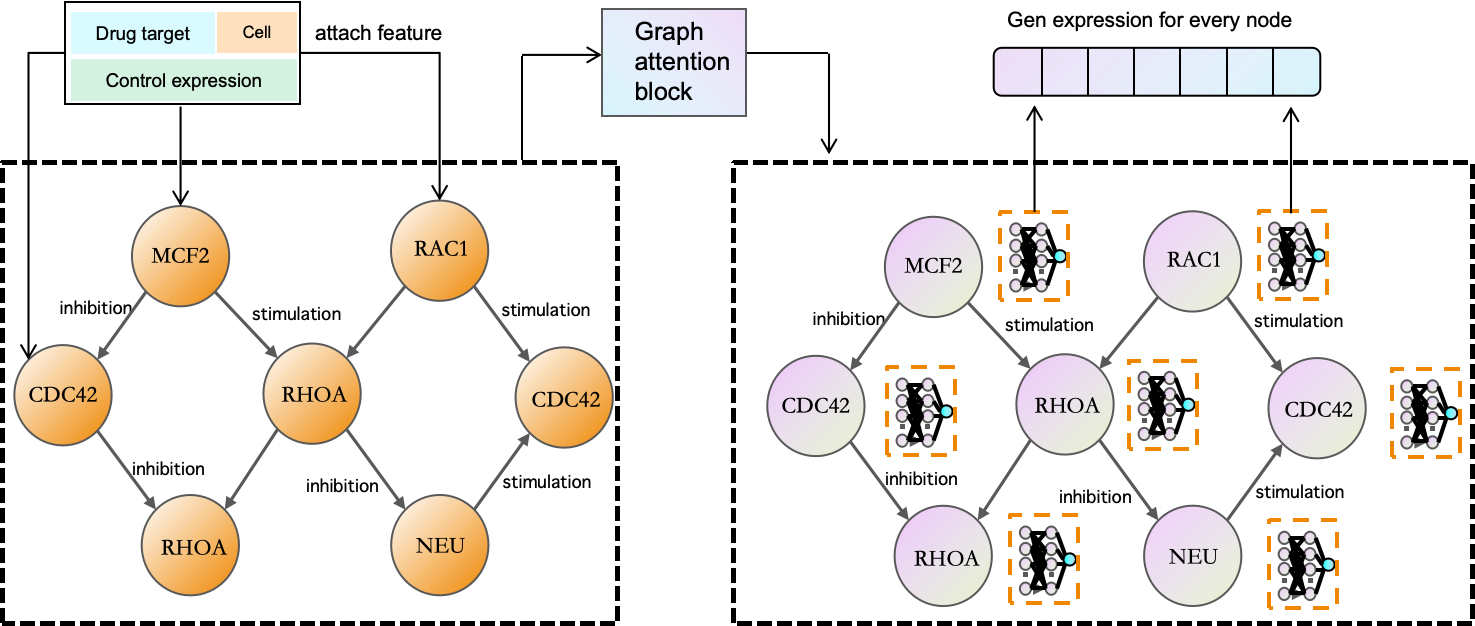
\includegraphics[width=0.95\linewidth]{figures/proposed_model.png}
    \caption{Structure of the proposed model. The model combines the biological interaction graph, the control profile, and drug target information to predict the gene wise response.}
    \label{fig:proposed_model}
\end{figure}

\noindent The proposed model predicts one response value for each gene. It uses a graph attention network on a biological interaction graph. The graph, node features, and cell information are introduced in the input section above.

\subsection{Node features}
The proposed model starts from one node per gene. The control profile provides one scalar input for each node. The drug target vector also provides one scalar input for each node. These two inputs are projected to a hidden dimension $F$. In the current main setting, $F=64$. The initial node representation matrix is
\begin{equation}
H^{(0)} \in \mathbb{R}^{G \times F}.
\end{equation}
\noindent More precisely, the control input and the drug target input are embedded separately, and the sample level fused cell context is added as an extra term:
\begin{equation}
H^{(0)} = \phi_{\mathrm{ctl}}(x_{\mathrm{ctl}}) + \phi_{\mathrm{drug}}(x_{\mathrm{drug}}) + c_{\mathrm{fused}}.
\end{equation}

\noindent For a mini batch, the node feature tensor becomes
\begin{equation}
H^{(0)} \in \mathbb{R}^{B \times G \times F}.
\end{equation}
\noindent When cell information is added at this stage, it changes what each node representation contains. It changes the sample specific state carried by each gene node before message passing starts.

\subsection{Graph multi-head attention block}
\noindent The backbone contains $L$ graph attention layers. In the main benchmark setting, $L=4$. Each layer uses multi head attention with $K=4$ heads. Since the hidden width is $F=64$, each head outputs $64/4=16$ features and the concatenated output returns to dimension 64. In the final model, cell information is not inserted directly into the attention score. Instead, the fused cell context is added to the node features before message passing starts. The attention block itself then follows the standard GAT style computation.

\noindent For each head, the node features are first projected linearly. The attention score for an edge is then computed from the transformed source and target node representations. A leaky ReLU is applied to this score, and the graph structure is used as a mask so that only existing edges receive nonzero attention. Softmax normalization is then applied over the neighbors of each node. The normalized attention weights are used to compute a weighted sum of neighbor features. After all heads are computed, their outputs are concatenated and passed through the activation function.

\noindent After the multi head attention update, the model applies dropout, a residual connection, and layer normalization. It then applies a position wise feed forward network, followed by a second dropout, a second residual connection, and a second layer normalization. The position wise feed forward network follows the Transformer design introduced by Vaswani et al.~\cite{vaswani2017attention}. It consists of two linear transformations with a ReLU activation in between. For a node representation $h_{v}$, this is computed as
\begin{equation}
\mathrm{FFN}(h_{v}) = W_{2} \max(0, W_{1} h_{v} + b_{1}) + b_{2}.
\end{equation}
Attention mixes information across connected nodes, while the feed forward network refines each node representation separately.

\begin{figure}[H]
    \centering
    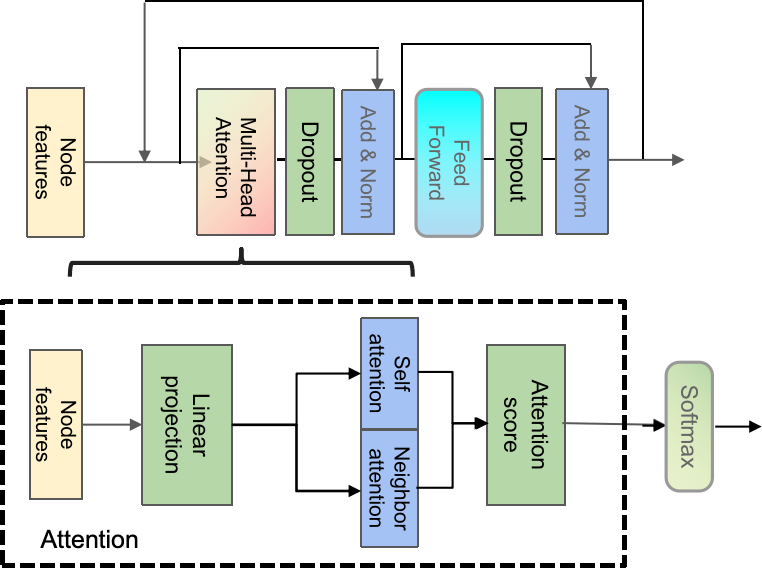
\includegraphics[width=0.70\linewidth]{figures/proposal_model_attneion.png}
    \caption{Flow of one graph attention block used in the proposed model. The input node features are linearly projected, standard graph attention scores are computed and normalized with softmax, and the multi head output is followed by dropout, residual addition, layer normalization, and a position wise feed forward network.}
    \label{fig:gat_flow}
\end{figure}

\noindent Figure~\ref{fig:gat_flow} shows the computation in one graph block. The block uses the node representations prepared in the input stage, which already contain the fused sample context. It then applies standard graph attention for neighbor aggregation. When several graph attention layers are stacked, the output of one block becomes the input to the next block.

\subsection{Output layer}
\noindent After the last graph layer, each node has a final hidden vector $h_{v}^{(L)} \in \mathbb{R}^{F}$. The output layer uses two parallel linear readouts. One predicts the mean response,
\begin{equation}
\mu_{v}=w_{\mu}^{\top} h_{v}^{(L)} + b_{\mu},
\end{equation}
and the other predicts a log variance term,
\begin{equation}
\log \sigma_{v}^{2}=w_{\sigma}^{\top} h_{v}^{(L)} + b_{\sigma},
\end{equation}
where $w_{\mu}, w_{\sigma} \in \mathbb{R}^{F}$ and $b_{\mu}, b_{\sigma} \in \mathbb{R}$. Stacking these outputs over all genes gives the full mean prediction $\mu \in \mathbb{R}^{G}$ and the full log variance prediction $\log \sigma^{2} \in \mathbb{R}^{G}$.

\noindent In the implementation, the readout is applied independently to each node. This design gives one mean value and one uncertainty related value for each gene node. At batch level, the output has shape $\mathbb{R}^{B \times G \times 2}$.

\subsection{Uncertainty}
\noindent Uncertainty estimation is an important part of the proposed model. The reason is that perturbation responses are not equally reliable across all genes or all samples. Some drug effects are strong and consistent, while others are weak, noisy, or highly dependent on cellular state in biological environment. Drug response is shaped by many factors such as baseline expression, pathway activity, hidden regulatory effects, and measurement noise. A single point estimate is therefore not always enough. The model should also indicate how certain it is about each predicted response.

\noindent In this thesis, the uncertainty output is based on a Gaussian view of the prediction target. Instead of treating the response of one gene as a single fixed value, the model treats it as a random variable with a distribution. For gene $g$ in sample $i$, the target response is modeled as
\begin{equation}
y_{ig} \sim \mathcal{N}(\mu_{ig}, \sigma_{ig}^{2}).
\end{equation}
Here $\mu_{ig}$ is the expected response and $\sigma_{ig}^{2}$ describes how uncertain the model is about that response. A small variance means that the model expects the target to stay close to the mean. A large variance means that the response is treated as less predictable.

\noindent For this reason, the output layer predicts two quantities for each gene. The first is the predictive mean $\mu_{v}$, which represents the expected perturbation response. The second is a log variance term $\log \sigma_{v}^{2}$, which represents predictive uncertainty in a numerically stable form. For one gene node, the output is
\begin{equation}
(\mu_{v}, \log \sigma_{v}^{2}),
\end{equation}
and stacking these values over all genes gives a batch level output of shape $\mathbb{R}^{B \times G \times 2}$. The mean branch gives the predicted response profile. The variance branch gives a gene wise estimate of how reliable that prediction is. A larger predicted variance means that the model treats that response as less certain.

\noindent This design also matches the biological setting more closely. A drug may have a clear effect on some genes and a more ambiguous effect on others. The same drug can also behave differently across cells when the baseline state changes. Predicting both a mean and a variance lets the model represent this uneven confidence directly, instead of forcing all genes to be treated as equally certain.

\subsection{Loss function}
\noindent The proposed model uses an uncertainty aware regression loss. Let $m \in \{0,1\}^{G}$ be a gene mask. The supervised target for gene $g$ in sample $i$ is compared with the predicted mean $\mu_{ig}$ and predicted log variance $\log \sigma_{ig}^{2}$. The masked Gaussian negative log likelihood is
\begin{equation}
\mathcal{L}_{\mathrm{nll}}=\frac{1}{B\sum_{g} m_{g}}\sum_{i=1}^{B}\sum_{g=1}^{G} m_{g}\,\frac{1}{2}\left[\log \sigma_{ig}^{2}+\frac{(y_{ig}-\mu_{ig})^{2}}{\sigma_{ig}^{2}}\right].
\end{equation}
This form follows directly from the Gaussian assumption introduced above. It is the negative log likelihood of observing the target response under the predicted mean and variance.
Here $B$ is the mini batch size and $G$ is the number of genes. The mask value $m_g$ indicates whether gene $g$ is included in the supervised loss. The term $y_{ig}$ is the true perturbation response for sample $i$ and gene $g$. The term $\mu_{ig}$ is the predicted mean response. The term $\sigma_{ig}^{2}$ is the predicted variance, and $\log \sigma_{ig}^{2}$ is used in the implementation for numerical stability. In the current landmark gene setting, the selected target genes match the prediction space, so the mask covers all selected genes.

\noindent The likelihood contains two parts. The squared error term $(y_{ig}-\mu_{ig})^{2}/\sigma_{ig}^{2}$ encourages the predicted mean to stay close to the target. Its contribution becomes larger when the model predicts a small variance, so confident predictions are required to be accurate. The $\log \sigma_{ig}^{2}$ term penalizes unnecessarily large uncertainty. These two parts work together. A large variance can reduce the normalized error term, but it also increases the log variance penalty. This balance prevents the model from assigning high uncertainty everywhere and encourages it to learn where the response is predictable and where it is less reliable.

\noindent The model also uses a sample wise Pearson correlation term. For one sample $i$, the correlation over the selected genes is
\begin{equation}
\mathrm{corr}\!\left(y_{i},\mu_{i}\right)=\frac{\sum_{g}\left(y_{ig}-\bar{y}_{i}\right)\left(\mu_{ig}-\bar{\mu}_{i}\right)}{\sqrt{\sum_{g}\left(y_{ig}-\bar{y}_{i}\right)^{2}}\sqrt{\sum_{g}\left(\mu_{ig}-\bar{\mu}_{i}\right)^{2}}},
\end{equation}
where $\bar{y}_{i}$ and $\bar{\mu}_{i}$ are means over the selected genes. The correlation loss is
\begin{equation}
\mathcal{L}_{\mathrm{pcc}} = 1-\frac{1}{B}\sum_{i=1}^{B}\mathrm{corr}\!\left(y_{i},\mu_{i}\right).
\end{equation}
This form is used because the training objective is minimized. A larger Pearson correlation should improve the model, so the optimization uses $1-\mathrm{PCC}$ rather than $\mathrm{PCC}$ itself. When the predicted response matches the true gene wise pattern more closely, the average correlation increases and $\mathcal{L}_{\mathrm{pcc}}$ becomes smaller.

The main prediction loss is
\begin{equation}
\mathcal{L}_{\mathrm{full}}=\mathcal{L}_{\mathrm{nll}}+\lambda_{\mathrm{pcc}}\mathcal{L}_{\mathrm{pcc}}.
\end{equation}
The likelihood term reduces mean prediction error while learning a gene wise uncertainty level. The PCC term encourages agreement in the shape of the response profile across genes. Together they encourage both an accurate response and a meaningful confidence estimate. In the implementation, $\lambda_{\mathrm{pcc}}=5$.

\noindent The model also uses a counterfactual drug loss. In each training step, one forward pass uses the true drug target vector and another uses a zero drug target vector. Let the second prediction loss be $\mathcal{L}_{\mathrm{cf}}$. The hinge penalty is
\begin{equation}
\mathcal{L}_{\mathrm{hinge}}=\max\!\left(0,\delta-\left(\mathcal{L}_{\mathrm{cf}}-\mathcal{L}_{\mathrm{full}}\right)\right).
\end{equation}
The final objective is
\begin{equation}
\mathcal{L}=\mathcal{L}_{\mathrm{full}}+\lambda_{\mathrm{cf}}\mathcal{L}_{\mathrm{hinge}}.
\end{equation}
This term encourages the factual prediction to be better than the counterfactual one~\cite{hadsell2006contrastive, schroff2015facenet, wachter2017counterfactual}.

\subsection{Optimization and Implementation Details}
The proposed model is trained with Adam. In the main benchmark setting, the learning rate is $5 \times 10^{-4}$. The training uses mini batches of size 32 and fixed training epochs. The main benchmark results use 50 epochs. In each training step, the loop computes one factual forward pass and one counterfactual forward pass. It then backpropagates the full counterfactual training objective. The training loop reports sample wise PCC and MSE after each epoch.

\noindent The complete model configuration and hyperparameters are summarized in Table~\ref{tab:proposed_model_config}. The node readout is applied independently to each gene node. The main drug input is the target based drug vector.

\begin{table}[H]
    \centering
    \caption{Main configuration of the proposed model.}
    \label{tab:proposed_model_config}
    \begin{tabular}{ll}
        \hline
        Setting & Value \\
        \hline
        Optimizer & Adam \\
        Learning rate & $5 \times 10^{-4}$ \\
        Batch size & 32 \\
        Training epochs & 50 \\
        Hidden dimension & 64 \\
        Graph attention layers & 4 \\
        Attention heads & 4 \\
        Dropout & 0.2 \\
        Output & Mean and log variance \\
        Log variance clip range & $[-6, 2]$ \\
        Pearson loss weight $\lambda_{\mathrm{pcc}}$ & 5 \\
        Counterfactual weight $\lambda_{\mathrm{cf}}$ & 1 \\
        Counterfactual margin $\delta$ & 0.1 \\
        \hline
    \end{tabular}
\end{table}

\noindent These values are kept the same across the main benchmark experiments unless otherwise stated.

\section{Base model}
\subsection{Architecture}
Figure~\ref{fig:base_model_structure} shows the benchmark model. The benchmark follows the DeepCOP style fully connected design~\cite{woo2020deepcop}. It does not use a biological interaction graph.

\begin{figure}[H]
    \centering
    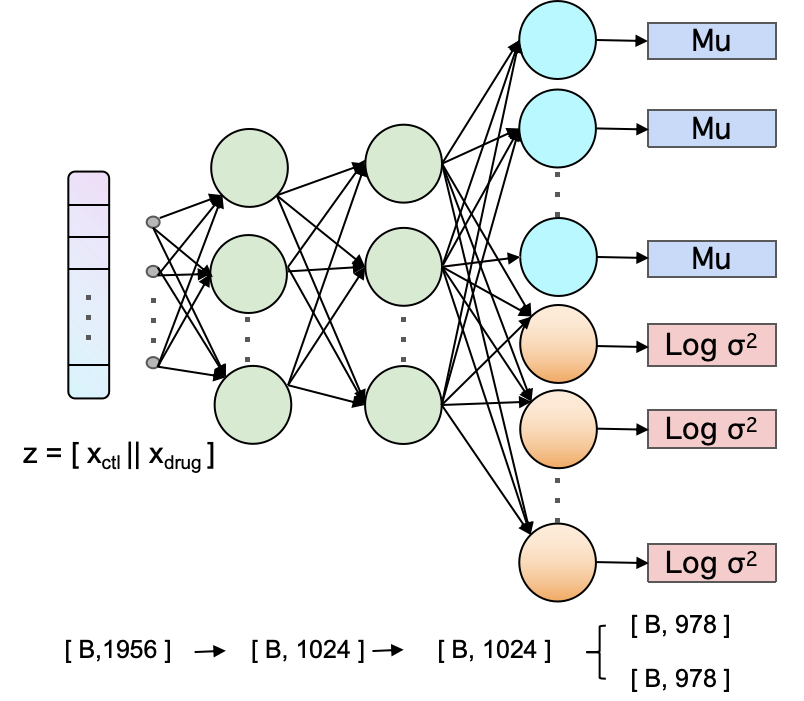
\includegraphics[width=0.95\linewidth]{figures/base_model_structure.png}
    \caption{Structure of the benchmark model. Control gene expression and drug features are concatenated and passed through a feed forward network to predict the response vector.}
    \label{fig:base_model_structure}
\end{figure}

\noindent The benchmark uses the shared control profile and drug input introduced above. The concatenated input is
\begin{equation}
z = [x_{\mathrm{ctl}} \Vert x_{\mathrm{drug}}] \in \mathbb{R}^{2G}.
\end{equation}
For a mini batch, the same input is written as $Z \in \mathbb{R}^{B \times 2G}$. The model then applies two fully connected blocks. Each block uses a dense layer, batch normalization, ReLU, and dropout. The current implementation uses a hidden width of 1024. This means that the hidden representation after each block has shape $\mathbb{R}^{B \times 1024}$. The output stage predicts a mean value and a log variance value for each gene. For one sample, the final output can be written as
\begin{equation}
\left[\mu, \log \sigma^{2}\right] \in \mathbb{R}^{G \times 2}.
\end{equation}
At batch level, the final output has shape $\hat{Y} \in \mathbb{R}^{B \times G \times 2}$.

\subsection{Loss function}
The benchmark model is trained with an uncertainty aware Gaussian negative log likelihood. In the current implementation, the training target is residualized by subtracting a cell specific mean response estimated from the training set. If this residual target is written as $y^{\prime} \in \mathbb{R}^{G}$, the training loss is
\begin{equation}
\mathcal{L}_{\mathrm{base}}=\frac{1}{BG}\sum_{i=1}^{B}\sum_{g=1}^{G}\frac{1}{2}\left[\log \sigma_{ig}^{2}+\frac{\left(y^{\prime}_{ig}-\mu_{ig}\right)^{2}}{\sigma_{ig}^{2}}\right],
\end{equation}
where $B$ is the mini batch size. Here $\mu_{ig}$ is the predicted mean response and $\sigma_{ig}^{2}$ is the predicted variance for gene $g$ in sample $i$. This loss keeps the benchmark model comparable to the proposed model at the output level, while the two architectures remain different.

\subsection{Optimization}
The benchmark model is trained with Adam. In the repository version used here, the learning rate is $5 \times 10^{-4}$. The training script uses mini batches of size 256 and fixed training epochs. The benchmark results in this thesis use 10 epochs. The script reports sample wise PCC and MSE on the training and validation sets after each epoch. These benchmark results are produced with the repository implementation rather than the original DeepCOP code base.

\section{Training and evaluation protocol}
The same target definition is used for both models, but the data pairing strategy differs between training and test. In training, one treatment profile can be matched to several controls. In test, each treatment profile is matched to one control. The split is applied before the final treatment control matching. After that step, the training and test control pools are separated. This design reduces leakage.

\noindent Three split settings are used. Warm split uses a random sample split. Cold drug split holds out test drugs from training. Cold cell split holds out test cell lines from training.

\noindent In this pipeline, the training set uses multiple matched controls for each treatment profile. The default number is three controls per treatment profile. If fewer controls are available, sampling is done with replacement. The test set uses one matched control for each treatment profile. This makes the test setting more conservative.

\noindent Performance is reported with mean squared error and sample wise Pearson correlation coefficient. In addition, this thesis also reports top gene precision and regulation sign accuracy in the results chapter. Attention weights from the proposed model are used only for interpretation. They are not used to change the prediction after training.
